\documentclass[11pt]{article}


% This must come after amsthm
% \usepackage{unicode-math}
% \setmainfont{Cambria}
% \setmathfont{XITS Math} % https://github.com/khaledhosny/xits
%                         % time-like math font, suitable with LuaLatex

\usepackage{fullpage}
\usepackage{amsmath} % \dfrac
\usepackage{graphicx}

\title{Back Propagation Algorithm}
\author{Feiyi Wang}
\date{}

\begin{document}
\maketitle

There are many tutorials on the subject, with different notations. This is one I feel most at home to use.

\section{Notation}

\begin{tabular}{@{}p{1in}p{4in}}
    $x_j^l$ & Input to node $j$ of layer $l$ \medskip \\

    $w_{ij}^{l}$ & Weight from layer $l-1$ node $i$ to layer $l$ at node $j$ \medskip \\

    $\sigma(x) = \tfrac{1}{1+e^{-x}}$ & Sigmoid function \medskip \\

    $b_j^{l}$ & Bias of node $j$ of layer $l$ \medskip \\

    $\mathcal{O}_{j}^{l}$ & Output of node $j$ in layer $l$ \medskip \\

    $t_j$ & Target value of node $j$ of the output layer \medskip \\


\end{tabular}


\section{Sigmoid and its derivatives}

\begin{equation}
    \sigma(x) = \frac{1}{1+e^{-x}}
\end{equation}

Its derivative:

\begin{align*}
\frac{d}{dx}\sigma(x) &= \frac{d}{dx} \left(\frac{1}{1+e^{-x}}\right) \\
    &= \frac{0 - (1+e^{-x})^\prime}{(1+e^{-x})^2} \\
    &= \frac{e^{-x}}{(1+e^{-x})^2} \\
    &= \frac{(1 + e^{-x}) - 1}{(1+e^{-x})^2} \\
    &= \frac{1+e^{-x}}{(1+e^{-x})^2} - \left( \frac{1}{1+e^{-x}} \right)^2 \\
    &= \sigma(x) - \sigma(x)^2  \\
    &= \sigma(x)(1-\sigma(x)) \\
\end{align*}

Finally, we have what we need:

\begin{equation}
\sigma^\prime(x) = \sigma(x)(1-\sigma(x))
\end{equation}


\section{Neuron with multiple inputs}

This figure illustrates how above notation and concepts connects on a neuron.

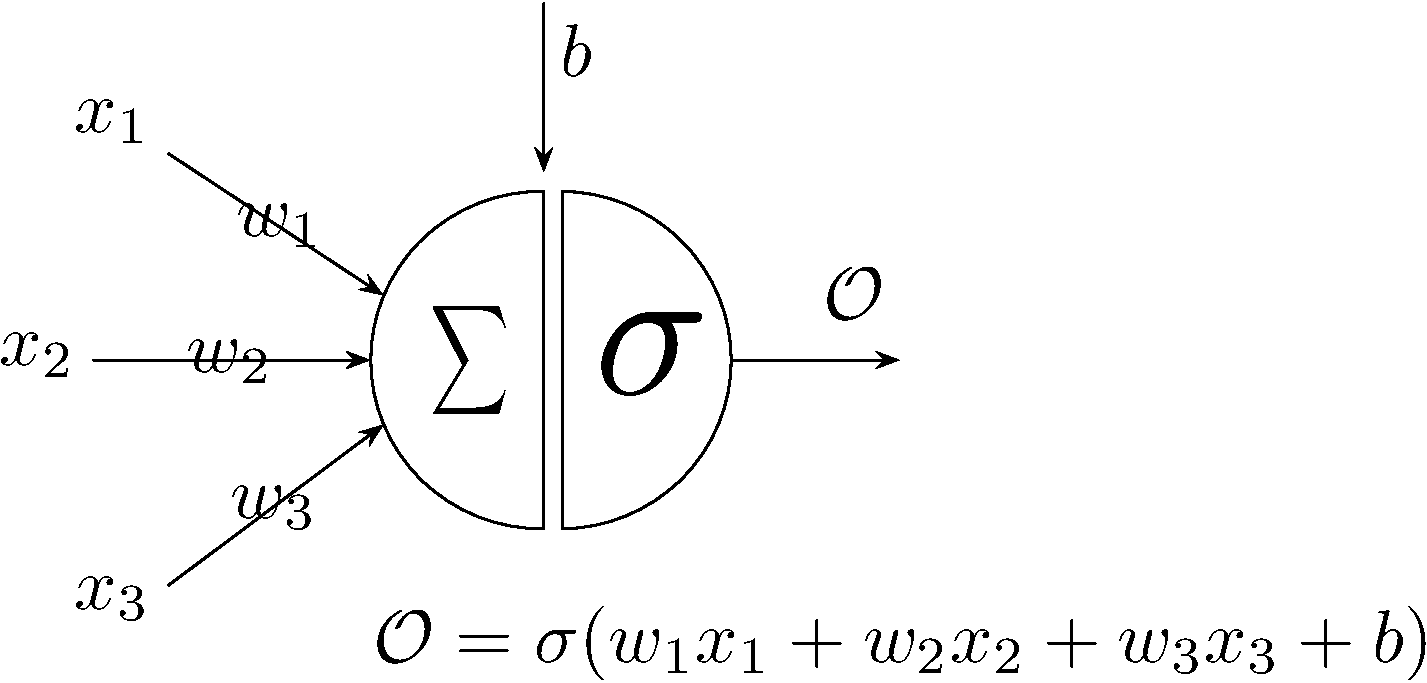
\includegraphics[width=3.5in]{neuron-connect.pdf}


\section{Error function}

The error function is defined as:

\begin{equation}
E = \frac{1}{2} \sum_{k \in K}(\mathcal{O}_k - t_k)^2
\end{equation}

Assume the output layer has $K$ output nodes, this error function sums up all the errors on each of the output node $k$, where $k \in K$.

Given this error function, we want to calculate:
\[ \frac{\partial E}{\partial w_{jk}^l} \]

The partial derivative reflects the rate of changes on error given a weight $w_{jk}^l$. Once we have this value, we can adjust $w_{jk}^l$ toward minimizing the error. To calculate this value, we consider two separate cases:

\begin{itemize}
\item the node is in output layer
\item the node is in hidden layer
\end{itemize}

\section{Error derivative for output layer node}

We are interested in partial derivative on the weight connecting node $j$ from previous layer to node $k$ of current and output layer, $w_{jk}$. Also to be clear, the left portion of the neuron, $\sum$ output is denoted by $x_k$, this is defined as:
\begin{equation}
\label{eq:xk}
x_k = \sum_{j \in H} \mathcal{O}_j w_{jk}
\end{equation}

where $H$ is the set of all nodes in the previous layer, and $\mathcal{O}_j$ is the output from a node $j$ in the previous layer. The same reasoning applies that $\mathcal{O}_k$ is the output of node $k$, and it is the $\sigma$ function applied to input $x_k$:

\begin{equation}
\mathcal{O}_k = \sigma(x_k)
\end{equation}




\begin{align*}
\frac{\partial E}{\partial w_{jk}}  &= \frac{\partial}{\partial w_{jk}}
            \frac{1}{2} \sum_{k\in K}(\mathcal{O}_k - t_k)^2 \\
        &= \frac{\partial E}{\partial w_{jk}} \frac{1}{2} (\mathcal{O}_k - t_k)^2 \\
        &= (\mathcal{O}_k - t_k) \frac{\partial}{\partial w_{jk}} \mathcal{O}_k && \text{$w_{jk}$ do not contribute error other than node $k$} \\
        &= (\mathcal{O}_k - t_k) \frac{\partial}{\partial w_{jk}} \sigma(x_k) \\
        &= (\mathcal{O}_k - t_k) \sigma^{\prime}(x_k) \frac{\partial}{\partial w_{jk}} x_k \\
        &= (\mathcal{O}_k - t_k) \sigma(x_k) (1-\sigma(x_k)) \frac{\partial}{\partial w_{jk}} x_k \\
        &= (\mathcal{O}_k - t_k) \sigma(x_k) (1-\sigma(x_k)) \mathcal{O}_j && \text{only $\mathcal{O}_j$ is left}\\
        &= (\mathcal{O}_k - t_k) \mathcal{O}_k (1-\mathcal{O}_k) \mathcal{O}_j \\
\end{align*}


We often define $\delta_k$ the collection of all terms involving $k$:

\begin{equation}
\delta_k = \mathcal{O}_k (1-\mathcal{O}_k) (\mathcal{O}_k - t_k)
\end{equation}

Then, we can rewrite the derivative as:

\begin{equation}
\frac{\partial E}{\partial w_{jk}} = \mathcal{O}_j \delta_k
\end{equation}


\section{Error derivation for the hidden layer node}

We now are interested in partial derivative on the weight connecting node $i$ from a previous layer to node $j$ of hidden layer, $w_{ij}$. Based on Eq.\ref{eq:xk}, we know that:
\begin{equation}
\label{eq:xk_prime}
\frac{\partial x_k}{\partial \mathcal{O}_j} = w_{jk}
\end{equation}

This results comes in handy below.


\begin{align*}
\frac{\partial E}{\partial w_{ij}}  &= \frac{\partial}{\partial w_{ij}}
            \frac{1}{2} \sum_{k\in K}(\mathcal{O}_k - t_k)^2 && \text{we can't drop $\sum$ anymore}\\
            &= \sum_{k\in K}(\mathcal{O}_k-t_k) \frac{\partial}{\partial w_{ij}}\mathcal{O}_k \\
            &= \sum_{k\in K}(\mathcal{O}_k-t_k) \frac{\partial}{\partial w_{ij}}\sigma(x_k)\\
            &= \sum_{k\in K}(\mathcal{O}_k-t_k) \sigma^{\prime}(x_k) \frac{\partial x_k}{\partial w_{ij}}
                && \text{chain rule} \\
            &= \sum_{k\in K}(\mathcal{O}_k-t_k) \sigma(x_k) (1-\sigma(x_k)) \frac{\partial x_k}{\partial w_{ij}}  \\
            &= \sum_{k\in K}(\mathcal{O}_k-t_k) \mathcal{O}_k (1-\mathcal{O}_k) \frac{\partial x_k}{\partial w_{ij}}
                && \text{replace $\sigma$ with $\mathcal{O}$ as before} \\
            &= \sum_{k\in K}(\mathcal{O}_k-t_k) \mathcal{O}_k (1-\mathcal{O}_k) \frac{\partial x_k}{\partial \mathcal{O}_j}
                \cdot \frac{\partial \mathcal{O}_j}{\partial w_{ij}} && \text{chain rule: $x_k$ depends on output of $\mathcal{O}_j$} \\
            &= \sum_{k\in K}(\mathcal{O}_k-t_k) \mathcal{O}_k (1-\mathcal{O}_k) w_{jk}
                \cdot \frac{\partial \mathcal{O}_j}{\partial w_{ij}} && \text{Use Eq.\ref{eq:xk_prime}} \\
            &= \frac{\partial \mathcal{O}_j}{\partial w_{ij}} \sum_{k\in K}(\mathcal{O}_k-t_k) \mathcal{O}_k (1-\mathcal{O}_k) w_{jk} && \text{Since last term is independent of $k$} \\
            &= \frac{\partial \sigma(x_j)}{\partial w_{ij}} \sum_{k\in K}(\mathcal{O}_k-t_k) \mathcal{O}_k (1-\mathcal{O}_k) w_{jk} \\
            &= \sigma^{\prime}(x_j) \frac{\partial x_j}{\partial w_{ij}} \sum_{k\in K}(\mathcal{O}_k-t_k) \mathcal{O}_k (1-\mathcal{O}_k) w_{jk} && \text{chain rule} \\
            &= \mathcal{O}_j (1-\mathcal{O}_j) \frac{\partial x_j}{\partial w_{ij}} \sum_{k\in K}(\mathcal{O}_k-t_k) \mathcal{O}_k (1-\mathcal{O}_k) w_{jk} \\
    &= \mathcal{O}_j (1-\mathcal{O}_j) \mathcal{O}_i \sum_{k\in K}(\mathcal{O}_k-t_k) \mathcal{O}_k (1-\mathcal{O}_k) w_{jk}
            && \text{input to node $j$ is output of $i$}\\
            &= \mathcal{O}_j (1-\mathcal{O}_j) \mathcal{O}_i \sum_{k\in K}\delta_k w_{jk} \\
\end{align*}

If we define all terms except $\mathcal{O}_i$ to be $\delta_j$, that is:

\begin{equation}
\delta_j = \mathcal{O}_j (1-\mathcal{O}_j)  \sum_{k\in K}\delta_k w_{jk}
\end{equation}

then we have:

\begin{equation}
\frac{\partial E}{\partial w_{ij}} = \mathcal{O}_i \delta_j
\end{equation}

\end{document}
